\section{附件}

\subsection{本地文件}

\begin{itemize}
	\item training.py:     训练模型代码
	\item training.ipynb:  代码同training.py,保存了输出内容
	\item inference.py:    使用模型进行预测代码
	\item inference.ipynb: 代码同inference.py,保存了输出内容
	\item result.csv:      保存了预测结果,raw\_id对应音频文件名,birds用空格分隔检测出的鸟类,鸟类名为\href{ebird.org}{ebird.org}中编码的,需要查看其学名可以通过访问ebird.org/species/[鸟名编码],在banner图片中查看到.如图所示:
	\begin{figure}[thbp!]
		\centering
		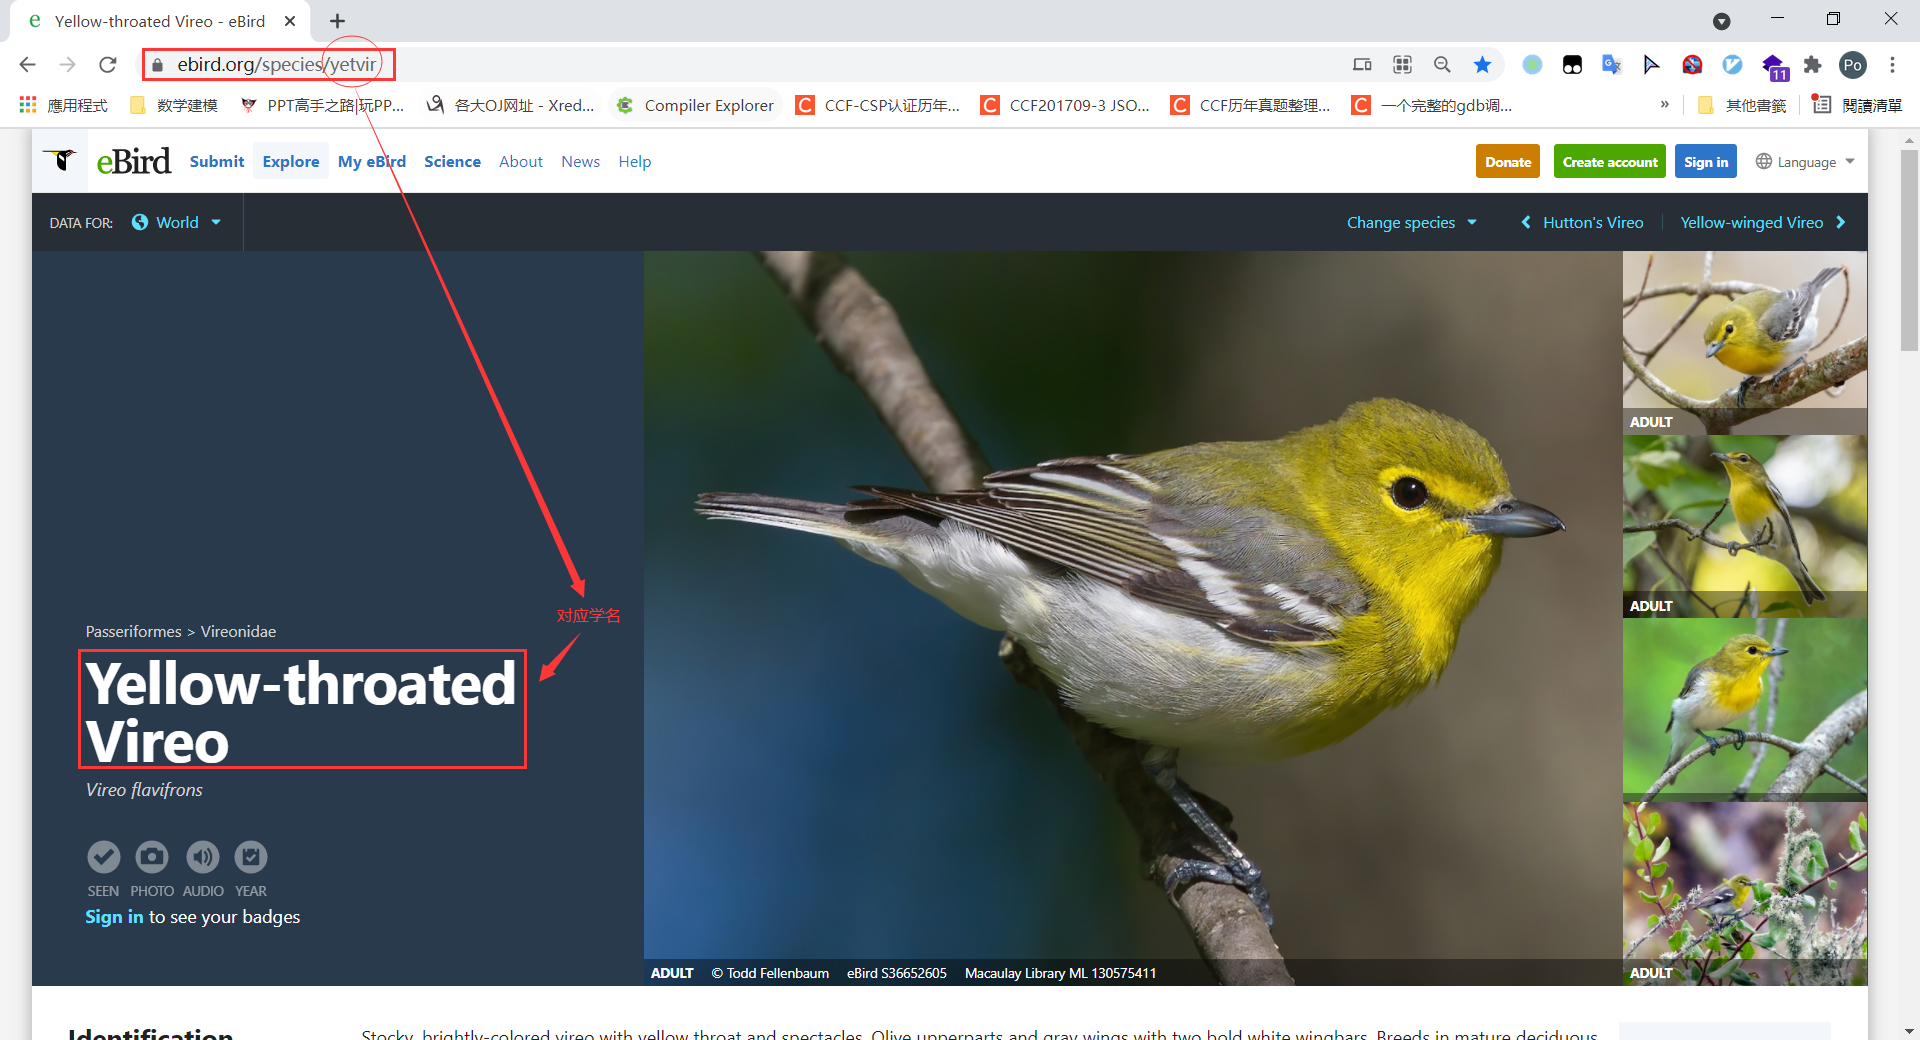
\includegraphics[scale=0.2]{figure/find_name}
		\caption{查看yetvir对应的学名为Yellow-throated Vireo}
	\end{figure}
\end{itemize}

\subsection{在线数据(点击文字超链接可达)}

\begin{itemize}
	\item \href{https://www.kaggle.com/c/birdsong-recognition}{Cornell Birdcall Identification鸟类识别比赛数据库}
	\item \href{https://www.kaggle.com/tsuipo/bird-pic}{自行从\href{ebird.org}{ebird.org}爬取后上传的鸟类图片}
\end{itemize}